\section{Setup}
% \vspace{-4.5mm}
% \vspace{-1em}
\begin{minted}[breaklines,frame=none,framesep=0pt]{json}
"shell_cmd": "g++ -std=c++17 -o \"$file_base_name\" \"$file\" && timeout 2.5s ./\"$file_base_name\" < input.txt > output.txt",
"file_regex": "^(..[^:]*):([0-9]+):?([0-9]+)?:? (.*)$",
"working_dir": "${file_path}",
"selector": "source.c, source.c++"
\end{minted}


\subsection{\small Sublime Build  \scriptsize}
\inputminted[breaklines, breakanywhere]{c++}{code/01-Setup/01-Sublime Build.cpp}

\subsection{\small Template  \scriptsize}
\inputminted[breaklines, breakanywhere]{c++}{code/01-Setup/02-Template.cpp}

\subsection{\small Input Gen  \scriptsize}
\inputminted[breaklines, breakanywhere]{c++}{code/01-Setup/03-Input Gen.cpp}

\subsection{\small Bash Script  \scriptsize}
\inputminted[breaklines, breakanywhere]{c++}{code/01-Setup/04-Bash Script.cpp}

% \vspace{0.2em}
% \vspace{-2.5mm}
\begin{minted}[breaklines,frame=none,framesep=0pt]{bash}
set -e
g++ code.cpp -o code
g++ gen.cpp -o gen
g++ brute.cpp -o brute
for((i = 1; ; ++i)); do
    ./gen $i > input_file
    ./code < input_file > myAnswer
    ./brute < input_file > correctAnswer
    diff -Z myAnswer correctAnswer > /dev/null || break
    echo "Passed test: "  $i
done
echo "WA on the following test:"
cat input_file
echo "Your answer is:"
cat myAnswer
echo "Correct answer is:"
cat correctAnswer
\end{minted}


\section{Number Theory}
\subsection{\small Euler Totient Function  \scriptsize}
\inputminted[breaklines, breakanywhere]{c++}{code/03-Number Theory/01-Euler Totient Function.cpp}

\subsection{\small Phi 1 to N  \scriptsize}
\inputminted[breaklines, breakanywhere]{c++}{code/03-Number Theory/02-Phi 1 to N.cpp}

\subsection{\small Segmented Sieve  \scriptsize}
\inputminted[breaklines, breakanywhere]{c++}{code/03-Number Theory/03-Segmented Sieve.cpp}

\subsection{\small Extended GCD  \scriptsize}
\inputminted[breaklines, breakanywhere]{c++}{code/03-Number Theory/04-Extended GCD.cpp}

\subsection{\small Linear Diophantine Equation  \scriptsize}
\inputminted[breaklines, breakanywhere]{c++}{code/03-Number Theory/05-Linear Diophantine Equation.cpp}

\subsection{\small Modular Inverse using EGCD  \scriptsize}
\inputminted[breaklines, breakanywhere]{c++}{code/03-Number Theory/06-Modular Inverse using EGCD.cpp}

\subsection{\small Exclusion DP  \scriptsize}
\inputminted[breaklines, breakanywhere]{c++}{code/03-Number Theory/07-Exclusion DP.cpp}

{\footnotesize
\begin{itemize}
    \item Here, 
    $f[i]$ = how many pairs/k-tuple such that their gcd is $i$ or it’s multiple (count of pairs those are divisible by $i$).
    \item $g[i]$ = how many pairs/k-tuple such that their gcd is $i$.
    \item $g[i]$ = $f[i] - \sum_{i \mid j} g[j]$.
    \item \textbf{Sum of all pair gcd:}

    We know, how many pairs are there such that their gcd is $i$ for every $i$ (1 to $n$). So now,  
    $\sum_{i=1}^{n} g[i] * i$.

    \item \textbf{Sum of all pair lcm $(1<=i,j<=n)$:}
    We know, 
    $\text{lcm}(a, b) = \frac{a * b}{\text{gcd}(a,b)}$. 
    \item Now, $f[i]$ = All pair product sum of those, whose gcd is $i$ or it’s multiple. 
    \item $g[i]$ = All pair product sum of those, whose gcd is $i$.
    \item $\text{Ans} = \sum_{i=1}^{n} \frac{g[i]}{i}$.

    \item All pair product sum = $(a_1 + a_2 + \cdots + a_n) * (a_1 + a_2 + \cdots + a_n)$
\end{itemize}
}

\subsection{\small Legendres Formula  \scriptsize}
\inputminted[breaklines, breakanywhere]{c++}{code/03-Number Theory/09-Legendres Formula.cpp}

\subsection{\small Binary Expo  \scriptsize}
\inputminted[breaklines, breakanywhere]{c++}{code/03-Number Theory/10-Binary Expo.cpp}

\subsection{\small Digit Sum of 1 to N  \scriptsize}
\inputminted[breaklines, breakanywhere]{c++}{code/03-Number Theory/11-Digit Sum of 1 to N.cpp}

\subsection{\small Pollard Rho  \scriptsize}
\inputminted[breaklines, breakanywhere]{c++}{code/03-Number Theory/12-Pollard Rho.cpp}

\subsection{\small [Problem] How Many Bases - UVa  \scriptsize}
\inputminted[breaklines, breakanywhere]{c++}{code/03-Number Theory/13-[Problem] How Many Bases - UVa.cpp}

\subsection{\small [Problem] Power Tower - CF  \scriptsize}
\inputminted[breaklines, breakanywhere]{c++}{code/03-Number Theory/14-[Problem] Power Tower - CF.cpp}

\subsection{\small Formula and Properties  \scriptsize}
\inputminted[breaklines, breakanywhere]{c++}{code/03-Number Theory/15-Formula and Properties.cpp}

{\footnotesize
\begin{itemize}
\item $\phi(n) = n \cdot \frac{p_1 - 1}{p_1} \cdot \frac{p_2 - 1}{p_2} \cdots$
\item $\phi(p^e) = p^e - \frac{p^e}{p} = p^e \cdot \frac{p-1}{p}$
\item For $n > 2$, $\phi(n)$ is always even.
\item $\sum_{d \mid n} \phi(d) = n$
\item NOD: $(e_1 + 1) \cdot (e_2 + 1) \cdots$
\item SOD: $\frac{p_1^{e_1 + 1} - 1}{p_1 - 1} \cdot \frac{p_2^{e_2 + 1} - 1}{p_2 - 1} \cdots$
% \item $\log(a \cdot b) = \log(a) + \log(b)$
% \item $\log(a^x) = x \cdot \log(a)$
% \item $\log_a(x) = \frac{\log_b(x)}{\log_b(a)}$
\item \footnotesize \textbf{Digit Count of n: } $\lfloor \log_{10}(n) \rfloor + 1$
\item \footnotesize \textbf{Arithmetic Progression Sum: } $\frac{n}{2} \cdot (a + p), \quad \frac{n}{2} \cdot (2a + (n-1)d)$
\item \footnotesize \textbf{Geometric Sum: } $S_n = a \cdot \frac{r^n - 1}{r - 1}$
\item $(1^2 + 2^2 + \cdots + n^2) = \frac{n (n + 1) (2n + 1)}{6}$
\item $(1^3 + 2^3 + \cdots + n^3) = \frac{n^2 (n + 1)^2}{4}$
\item $(2^2 + 4^2 + \cdots + (2n)^2) = \frac{2 n (n + 1) (2n + 1)}{3}$
\item $(1^2 + 3^2 + \cdots + (2n - 1)^2) = \frac{n (2n - 1) (2n + 1)}{3}$
\item $(2^3 + 4^3 + \cdots + (2n)^3) = 2 n^2 (n + 1)^2$
\item $(1^3 + 3^3 + \cdots + (2n - 1)^3) = n^2 (2n^2 - 1)$
\item For any number $n$ and bases $> \sqrt{n}$, there will be no representation where the number contains 0 at its second least significant digit. So it is enough to check for bases $\le \sqrt{n}$.
\item For some $x$ and $y$, let's try to find all $m$ such that $x \bmod m \equiv y \bmod m$. We can rearrange the equation into $(x - y) \equiv 0 \pmod{m}$. Thus, if $m$ is a factor of $|x - y|$, then $x$ and $y$ will be equal modulo $m$.
\end{itemize}
}


\section{Combinatorics and Probability}
\subsection{\small Combinations  \scriptsize}
\inputminted[breaklines, breakanywhere]{c++}{code/04-Combinatorics and Probability/01-Combinations.cpp}

\subsection{\small nCr for any mod  \scriptsize}
\inputminted[breaklines, breakanywhere]{c++}{code/04-Combinatorics and Probability/02-nCr for any mod.cpp}

\subsection{\small nCr without mod in O(r)  \scriptsize}
\inputminted[breaklines, breakanywhere]{c++}{code/04-Combinatorics and Probability/03-nCr without mod in O(r).cpp}

\subsection{\small Lucas Theorem  \scriptsize}
\inputminted[breaklines, breakanywhere]{c++}{code/04-Combinatorics and Probability/04-Lucas Theorem.cpp}

\subsection{\small Catalan Number  \scriptsize}
\inputminted[breaklines, breakanywhere]{c++}{code/04-Combinatorics and Probability/05-Catalan Number.cpp}

\subsection{\small Derangement  \scriptsize}
\inputminted[breaklines, breakanywhere]{c++}{code/04-Combinatorics and Probability/06-Derangement.cpp}

\subsection{\small Stars and Bars Theorem  \scriptsize}
\inputminted[breaklines, breakanywhere]{c++}{code/04-Combinatorics and Probability/07-Stars and Bars Theorem.cpp}

\vspace{-4.5mm}
{\footnotesize
\begin{itemize}
% \vspace{-1.5em}
\item Find the number of $k$-tuples of non-negative integers whose sum is $n$. \quad $\binom{n+k-1}{n}$
\item Find the number of $k$-tuples of non-negative integers whose sum is $\le n$. \quad $\binom{n+k}{k}$
\item Combination with Repetition (choose $k$ elements from $n$ objects, same element can be chosen multiple times). \quad $\binom{n+k-1}{k}$
\item How many ways to go from $(0,0)$ to $(n,m)$. \quad $\binom{n+m}{m}$
\end{itemize}\medskip\medskip\medskip
\textbf{Pascals Triangle is equivalent to nCr:}
\begin{center}
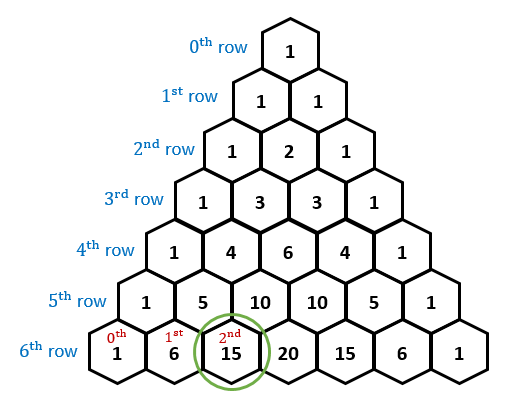
\includegraphics[width=0.5\linewidth]{images/pascals-triangle.png}
\end{center}
}


\subsection{\small Properties of Pascal's Triangle  \scriptsize}
\inputminted[breaklines, breakanywhere]{c++}{code/04-Combinatorics and Probability/09-Properties of Pascal's Triangle.cpp}

\vspace{-4.5mm}
{\footnotesize
\begin{itemize}
% \vspace{-1.5em}
\item $(a+b)^n = \sum_{k=0}^{n} \binom{n}{k} a^k b^{\,n-k}$ 
\item $(k+1)^n = \sum_{i=0}^{n} k^i \cdot \binom{n}{i}$ 
\item $\displaystyle \sum_{i=0}^{n} \binom{n}{i} = 2^n$ 
\item $\binom{n}{k} = \frac{n}{k} \binom{n-1}{k-1}$ 
\item $\displaystyle \sum_{k=0}^{m} \binom{n+k}{k} = \binom{n+m+1}{m}$ 
\item $\binom{n}{0}^2 + \binom{n}{1}^2 + \cdots + \binom{n}{n}^2 = \binom{2n}{n}$
\item $1\binom{n}{1} + 2\binom{n}{2} + \cdots + n\binom{n}{n} = n \, 2^{\,n-1}$ 
\end{itemize}
}

\subsection{\small Contribution Technique  \scriptsize}
\inputminted[breaklines, breakanywhere]{c++}{code/04-Combinatorics and Probability/11-Contribution Technique.cpp}

\vspace{-4.5mm}
{\footnotesize
\begin{itemize}
\item Sum of all pair sums: $\sum_{i=1}^{n} \sum_{j=1}^{n} (a_i + a_j)$\\
Every element will be added $2n$ times.
$\sum_{i=1}^{n} (2 \times n \times a_{i}) = 2 \times n \times \sum_{i=1}^{n} a_{i}.$
\item Sum of all subarray sums — \\
$\sum_{i=1}^{n} \left(a_{i} \times i \times (n - i + 1)\right).$
\item Sum of all Subsets sums —
$\sum_{i=1}^{n} \left(2^{n-1} \times a_{i}\right).$
\item Product of all pair product —
$\prod_{i=1}^{n} \left(a_{i}^{2 \times n}\right).$
\item XOR of subarray XORS — How many subarrays does an element have? ($i \cdot (n - i + 1)$ times). If subarray count is odd then this element can contribute in total XORs.
\item Sum of max minus min over all subset — Sort the array. $Min = 2^{\,n-i}, \ Max = 2^{\,i-1}$. $\sum_{i=1}^{n} \big(a_i \cdot 2^{\,i-1} - a_i \cdot 2^{\,n-i}\big)$
\item Sum using bits —
$\sum_{k=0}^{30} \left(cnt_{k}[1] \times 2^{k}\right).$
\item Sum of Pair XORs — XOR will 1 if two bits
are different
$\sum_{k=0}^{30} \left(cnt_{k}[0] \times cnt_{k}[1] \times 2^{k}\right).$
\item Sum of Pair ANDs — 
$\sum_{k=0}^{30} \left(cnt_{k}[1]^2 \times 2^{k}\right).$
\item Sum of Pair ORs — \\
$\sum_{k=0}^{30} \left( \left( cnt_{k}[1]^{2} + 2 \times cnt_{k}[1] \times cnt_{k}[0] \right) \times 2^{k} \right).$
\item Sum of Subset XORs — where $cnt0 != 0$
$\sum_{k=0}^{30} \left(2^{cnt_{k}[1] + cnt_{k}[0] - 1} \times 2^{k}\right).$
\item Sum of Subset ANDs — 
$\sum_{k=0}^{30} \left( \left(2^{cnt_{k}[1]} - 1\right) \times 2^{k} \right).$
\item Sum of Subset ORs — \\
$\sum_{k=0}^{30} \left( \left(2^{n} - 2^{cnt_{k}[0]}\right) \times 2^{k} \right).$
\item Sum of subarray XORs — Convert to prefix xor, then solve for pairs.
\item Sum of product of all subsequence — $\prod_{i=1}^{n} (a_i+1)-1$.
Example array — $[a,b]$ the subsequences are $\{a\}, \{b\}, \{a,b\}$ so ans is $a + b + (a \cdot b)$
\end{itemize}
}


\subsection{\small Probability and Expected Value  \scriptsize}
\inputminted[breaklines, breakanywhere]{c++}{code/04-Combinatorics and Probability/16-Probability and Expected Value.cpp}

\vspace{-5.5mm}
{\footnotesize
\begin{itemize}
\item Expected Value: $E = \frac{\text{Sum of all possible values}}{\text{Total number of outcomes}}$
\item Expected Value: $E = \sum_{i=1}^{n} P_i \cdot i$
\item Variance: $V(x) = E(x^2) - \{E(x)\}^2$
\item Expected Value with DP: $E(i) = \sum P(i \to j) \times (R(i \to j) + E(j))$ Where $R()$ is Immediate Reward(cost/count)
\item {
    Linearity of Expectation: 
    \begin{itemize}
    \item $E[X + Y] = E[X] + E[Y]$
    \item $E[\text{Total}] = E[I_1] + E[I_2] + \dots = \sum P(I_i=1)$
    \end{itemize}

    We need to define the Indicator Random Variable (I) correctly. Some Examples below —

    \textbf{Problem-1:} Find $E[\text{correct hats}]$ in a random permutation. Indicator $I_i$: "Does person $i$ get their own hat?"\\
    \textbf{Problem-2:} Find $E[\text{total inversions}]$ in a random permutation. Indicator $I_{ij}$: "Is pair $(i, j)$ an inversion?"\\
    \textbf{Problem-3:} Given a string $S$, delete a random index until it becomes empty. Find the expected count of palindromes seen (exclude $S$, include empty string). Indicator $I_L$: "Is the string of length $L$ a palindrome?"\\
    \textbf{Problem-4:} Pick $N$ random integers from $[1, k]$. Merge consecutive equal values (e.g., $1,1,2,2,1,1 \to 1,2,1$). Find the expected final length. Indicator $I_i$: "Is item $i$ different from item $i-1$?"
}
\item To get two consecutive heads, what is the expected number of tosses?
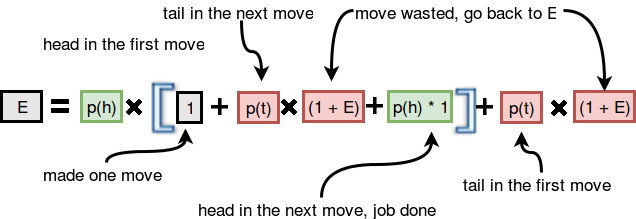
\includegraphics[width=0.9\linewidth]{images/expected_value_1.png}
\item To get $n$ heads, what is the expected number of tosses? Let’s define: to get $n$ heads, we need to toss $E(n)$ times. Now — I can get a head; I need to toss $E(n-1)$ more times, or if I get a tail; I need to toss $E(n)$ times. So, the recurrence is: $E(n) = 0.5 \cdot (1 + E(n-1)) + 0.5 \cdot (1 + E(n))$
% 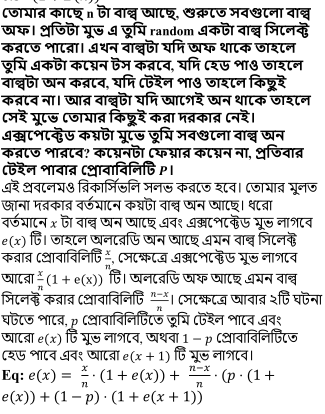
\includegraphics[width=\linewidth]{images/expected_value_2.png}
\item {
    You have $n$ bulbs, all of which are initially off. In each move, you randomly select one bulb. If the selected bulb is \textbf{off}, you toss a coin:
    \begin{itemize}
        \item If you get head, you turn it on.
        \item If you get tail, you do nothing.
    \end{itemize}

    If the bulb is already \textbf{on}, you skip that move (nothing happens).

    \par % Use par for a clean paragraph break
    Now, what is the expected number of moves required to turn all bulbs on?

    The coin is not fair — the probability of getting tail is $p$.
    This problem can also be solved recursively.

    \par
    Let's assume at some moment, $x$ bulbs are already on, and the expected number of moves needed from here is $e(x)$.

    The probability of picking an already on bulb is $\frac{x}{n}$.
    In that case, the expected number of moves is $\frac{x}{n} \times (1 + e(x))$.

    The probability of picking an off bulb is $\frac{n-x}{n}$.

    \par
    Now two things can happen:
    \begin{itemize}
        \item With probability $p$, you get tail, so you stay at the same state ($e(x)$ more moves).
        \item With probability $(1-p)$, you get head, so one more bulb turns on ($e(x+1)$ moves from there).
    \end{itemize}

    \par
    So, the recurrence relation is:
    \begin{align*}
    e(x) &= \frac{x}{n} (1 + e(x)) + \\
         & \quad \frac{n-x}{n} \big( p(1 + e(x)) + (1-p)(1 + e(x+1)) \big)
    \end{align*}
}
\end{itemize}
}


\subsection{\small Stirling Number of the First Kind  \scriptsize}
\inputminted[breaklines, breakanywhere]{c++}{code/04-Combinatorics and Probability/18-Stirling Number of the First Kind.cpp}

{\footnotesize
\begin{itemize}
    \item Count permutation according to their number of cycles.

    \item $S(n,k)$ counts the number of permutations of $n$ elements with $k$ disjoint cycles.

    \item $S(n,k) = (n-1) S(n-1,k) + S(n-1,k-1)$,\quad
          $S(0,0)=1$, \ $S(n,0)=S(0,n)=0$

    \item $S(n,1) = (n-1)!$

    \item $S(n,n-1) = \binom{n}{2}$

    \item $\displaystyle \sum_{k=0}^{n} S(n,k) = n!$
\end{itemize}
}

\subsection{\small Stirling Number of the Second Kind  \scriptsize}
\inputminted[breaklines, breakanywhere]{c++}{code/04-Combinatorics and Probability/20-Stirling Number of the Second Kind.cpp}

{\footnotesize
\begin{itemize}
    \item Number of ways to partition a set of $n$ objects into $k$ non-empty subsets.

    \item $S(n,k) = k\, S(n-1,k) + S(n-1,k-1)$,\quad
          $S(0,0)=1$, \ $S(n,0)=S(0,n)=0$

    \item $S(n,2) = 2^{n-1} - 1$

    \item $\displaystyle S(n,k) = \frac{1}{k!} \sum_{j=0}^{k} (-1)^{k-j} \binom{k}{j} j^{n}$

    \item $S(n,k) \cdot k!$ = number of ways to color $n$ nodes using colors from $1$ to $k$ such that each color is used at least once.
\end{itemize}

}

\section{Data Structure}
\subsection{\small Next Greater using Stack  \scriptsize}
\inputminted[breaklines, breakanywhere]{c++}{code/05-Data Structure/01-Next Greater using Stack.cpp}

\subsection{\small Segment Tree Lazy  \scriptsize}
\inputminted[breaklines, breakanywhere]{c++}{code/05-Data Structure/02-Segment Tree Lazy.cpp}

\subsection{\small First Element Greater than K in a Range  \scriptsize}
\inputminted[breaklines, breakanywhere]{c++}{code/05-Data Structure/03-First Element Greater than K in a Range.cpp}

\subsection{\small Number of Unique Element in a Range  \scriptsize}
\inputminted[breaklines, breakanywhere]{c++}{code/05-Data Structure/04-Number of Unique Element in a Range.cpp}

\subsection{\small Max Subarray Sum in a Range  \scriptsize}
\inputminted[breaklines, breakanywhere]{c++}{code/05-Data Structure/05-Max Subarray Sum in a Range.cpp}

\subsection{\small Count of subarrays such that their XOR is 0 in a range with upd  \scriptsize}
\inputminted[breaklines, breakanywhere]{c++}{code/05-Data Structure/06-Count of subarrays such that their XOR is 0 in a range with upd.cpp}

\subsection{\small Range Add, Set and Sum  \scriptsize}
\inputminted[breaklines, breakanywhere]{c++}{code/05-Data Structure/07-Range Add, Set and Sum.cpp}

\subsection{\small  a[i] = a[i] * b + c in a Range  \scriptsize}
\inputminted[breaklines, breakanywhere]{c++}{code/05-Data Structure/08- a[i] = a[i] * b + c in a Range.cpp}

\subsection{\small [Trick] Historic Information - GSS2  \scriptsize}
\inputminted[breaklines, breakanywhere]{c++}{code/05-Data Structure/09-[Trick] Historic Information - GSS2.cpp}

\subsection{\small [Problem] Strongest Community - LOJ  \scriptsize}
\inputminted[breaklines, breakanywhere]{c++}{code/05-Data Structure/10-[Problem] Strongest Community - LOJ.cpp}

\subsection{\small [Problem] Diablo - LOJ  \scriptsize}
\inputminted[breaklines, breakanywhere]{c++}{code/05-Data Structure/11-[Problem] Diablo - LOJ.cpp}

\subsection{\small Merge Sort Tree with Point Upd  \scriptsize}
\inputminted[breaklines, breakanywhere]{c++}{code/05-Data Structure/15-Merge Sort Tree with Point Upd.cpp}

\subsection{\small Sparse Table  \scriptsize}
\inputminted[breaklines, breakanywhere]{c++}{code/05-Data Structure/16-Sparse Table.cpp}

\subsection{\small DSU  \scriptsize}
\inputminted[breaklines, breakanywhere]{c++}{code/05-Data Structure/17-DSU.cpp}

\subsection{\small MOs Algorithm  \scriptsize}
\inputminted[breaklines, breakanywhere]{c++}{code/05-Data Structure/18-MOs Algorithm.cpp}

\subsection{\small MOs with Updates  \scriptsize}
\inputminted[breaklines, breakanywhere]{c++}{code/05-Data Structure/19-MOs with Updates.cpp}

\subsection{\small Persistent Segment Tree  \scriptsize}
\inputminted[breaklines, breakanywhere]{c++}{code/05-Data Structure/21-Persistent Segment Tree.cpp}

\subsection{\small Trie for bit  \scriptsize}
\inputminted[breaklines, breakanywhere]{c++}{code/05-Data Structure/24-Trie for bit.cpp}

\subsection{\small 2D BIT  \scriptsize}
\inputminted[breaklines, breakanywhere]{c++}{code/05-Data Structure/25-2D BIT.cpp}

\subsection{\small 2D Segment Tree  \scriptsize}
\inputminted[breaklines, breakanywhere]{c++}{code/05-Data Structure/26-2D Segment Tree.cpp}

\section{Dynamic Programming}
\subsection{\small Knapsack 2  \scriptsize}
\inputminted[breaklines, breakanywhere]{c++}{code/06-Dynamic Programming/01-Knapsack 2.cpp}

\subsection{\small LIS using Segment Tree  \scriptsize}
\inputminted[breaklines, breakanywhere]{c++}{code/06-Dynamic Programming/02-LIS using Segment Tree.cpp}

\subsection{\small Digit DP  \scriptsize}
\inputminted[breaklines, breakanywhere]{c++}{code/06-Dynamic Programming/03-Digit DP.cpp}

\subsection{\small Bitmask DP  \scriptsize}
\inputminted[breaklines, breakanywhere]{c++}{code/06-Dynamic Programming/04-Bitmask DP.cpp}

\subsection{\small MCM DP  \scriptsize}
\inputminted[breaklines, breakanywhere]{c++}{code/06-Dynamic Programming/05-MCM DP.cpp}

\subsection{\small Number of Unique Subsequence  \scriptsize}
\inputminted[breaklines, breakanywhere]{c++}{code/06-Dynamic Programming/06-Number of Unique Subsequence.cpp}

\subsection{\small [Problem] Rose Land - SUST 24  \scriptsize}
\inputminted[breaklines, breakanywhere]{c++}{code/06-Dynamic Programming/07-[Problem] Rose Land - SUST 24.cpp}

\subsection{\small DP with DS  \scriptsize}
\inputminted[breaklines, breakanywhere]{c++}{code/06-Dynamic Programming/10-DP with DS.cpp}

\subsection{\small [Problem] Sub-Palindromic Tree  \scriptsize}
\inputminted[breaklines, breakanywhere]{c++}{code/06-Dynamic Programming/15-[Problem] Sub-Palindromic Tree.cpp}

\subsection{\small SOS DP  \scriptsize}
\inputminted[breaklines, breakanywhere]{c++}{code/06-Dynamic Programming/16-SOS DP.cpp}

\section{Graph Theory}
\subsection{\small Binary Lifting and LCA  \scriptsize}
\inputminted[breaklines, breakanywhere]{c++}{code/07-Graph Theory/01-Binary Lifting and LCA.cpp}

\subsection{\small LCA and Sparse Table on Tree  \scriptsize}
\inputminted[breaklines, breakanywhere]{c++}{code/07-Graph Theory/02-LCA and Sparse Table on Tree.cpp}

\subsection{\small Dijkstra  \scriptsize}
\inputminted[breaklines, breakanywhere]{c++}{code/07-Graph Theory/03-Dijkstra.cpp}

\subsection{\small Bellman Ford  \scriptsize}
\inputminted[breaklines, breakanywhere]{c++}{code/07-Graph Theory/04-Bellman Ford.cpp}

\subsection{\small Floyd Warshall  \scriptsize}
\inputminted[breaklines, breakanywhere]{c++}{code/07-Graph Theory/05-Floyd Warshall.cpp}

\subsection{\small Strongly Connected Components  \scriptsize}
\inputminted[breaklines, breakanywhere]{c++}{code/07-Graph Theory/06-Strongly Connected Components.cpp}

\subsection{\small Articulation Points  \scriptsize}
\inputminted[breaklines, breakanywhere]{c++}{code/07-Graph Theory/07-Articulation Points.cpp}

\subsection{\small Find Bridges  \scriptsize}
\inputminted[breaklines, breakanywhere]{c++}{code/07-Graph Theory/08-Find Bridges.cpp}

\subsection{\small DSU on Tree  \scriptsize}
\inputminted[breaklines, breakanywhere]{c++}{code/07-Graph Theory/09-DSU on Tree.cpp}

\subsection{\small Heavy-Light Decomposition  \scriptsize}
\inputminted[breaklines, breakanywhere]{c++}{code/07-Graph Theory/10-Heavy-Light Decomposition.cpp}

\subsection{\small Inverse Graph  \scriptsize}
\inputminted[breaklines, breakanywhere]{c++}{code/07-Graph Theory/11-Inverse Graph.cpp}

\subsection{\small [Problem] Rooted Tree - Hackerrank  \scriptsize}
\inputminted[breaklines, breakanywhere]{c++}{code/07-Graph Theory/12-[Problem] Rooted Tree - Hackerrank.cpp}

{\footnotesize
Given a rooted tree, Upd: Add $d*k$ on $v$(subtree nodes of $u$), where $k$ will be given and $d$ is distance of $v$ from $u$. Query: Node Value/Subtree Sum (using ETT) or Path Value Sum (using HLD).
\textbf{Idea:} $d_i=$ dis from root to $i$. Then, $\text{ans} = k \cdot \sum_{v \in \text{subtree}(u)} d_v$. It's hard to find $d_v$ for each $u$, rather we can find $d_v=$ dis of $v$ from root. Although some extra value added on each $v$ of subtree $u$ because of $d_v$ from root (not $u$), we can easily subtract them ($depth[u]*k$).
}

\subsection{\small Dinic  \scriptsize}
\inputminted[breaklines, breakanywhere]{c++}{code/07-Graph Theory/16-Dinic.cpp}

\subsection{\small Flow Properties  \scriptsize}
\inputminted[breaklines, breakanywhere]{c++}{code/07-Graph Theory/17-Flow Properties.cpp}

\vspace{-5.5mm}
{\footnotesize
\begin{itemize}
\item \textbf{Bipartite Matching} = bpm
\item \textbf{Maximum Independent Set} = n - bpm. Bipartite Graph e min je koyta node remove korle kono edge thakbe na tar man bpm. segula bade baki node gula Independent jar man n - bpm.
\item \textbf{Vertex Cover} = bpm. Bipartite Graph e min je koyta vertex choose korle sob edge thakbe.
\item \textbf{Edge Cover} = n - bpm. Bipartite Graph e min je koyta edge choose korle sob vertex kono ekta edge er sathe connected thakbe.

\end{itemize}
}


\section{String}
\subsection{\small Hashing  \scriptsize}
\inputminted[breaklines, breakanywhere]{c++}{code/08-String/01-Hashing.cpp}

\subsection{\small Hashing with Updates  \scriptsize}
\inputminted[breaklines, breakanywhere]{c++}{code/08-String/02-Hashing with Updates.cpp}

\subsection{\small Hashing with Upd and Deletes  \scriptsize}
\inputminted[breaklines, breakanywhere]{c++}{code/08-String/03-Hashing with Upd and Deletes.cpp}

\subsection{\small Hashing on Tree  \scriptsize}
\inputminted[breaklines, breakanywhere]{c++}{code/08-String/04-Hashing on Tree.cpp}

\subsection{\small Compare 2 strings Lexicographically   \scriptsize}
\inputminted[breaklines, breakanywhere]{c++}{code/08-String/05-Compare 2 strings Lexicographically .cpp}

\subsection{\small KMP  \scriptsize}
\inputminted[breaklines, breakanywhere]{c++}{code/08-String/06-KMP.cpp}

\subsection{\small KMP Automata  \scriptsize}
\inputminted[breaklines, breakanywhere]{c++}{code/08-String/07-KMP Automata.cpp}

\subsection{\small Prefix Occurance Count  \scriptsize}
\inputminted[breaklines, breakanywhere]{c++}{code/08-String/08-Prefix Occurance Count.cpp}

\subsection{\small Number of palindormic substring in L to R using Wavelet Tree  \scriptsize}
\inputminted[breaklines, breakanywhere]{c++}{code/08-String/09-Number of palindormic substring in L to R using Wavelet Tree.cpp}

{\footnotesize
{
    It is easier to explain by considering only palindromes centered at indicies (so, odd length), the idea is the same anyway. For each index $i$, $r_i$ will be the longest radius of a palindrome centered there (in other words, the amount of palindromes centered at index $i$). Directly from manacher, this takes $\mathcal{O}(n)$ to calculate. \\

For a query $[l, r]$, we first compute $m = \frac{l+r}{2}$. Now we want to calculate
\begin{align*}
    \sum_{i=l}^{m} \min(i - l + 1, r_i) + 
    \sum_{i=m+1}^{r} \min(r - i + 1, r_i) \\
    \sum_{i=l}^{m} \min(i - l + 1, r_i) =
    \sum_{i=l}^{m} i + \min(1 - l, r_i - i).
\end{align*}
The sum over $i$ can be found in constant time. As for the other term, if we create some array $r'_{i} = r_i - i$ during the preprocessing, then the queries are asking for some over range of $\min(C, r'_{i})$ where $C$ is constant. You can solve this in $\mathcal{O}(\log n)$ per query using wavelet tree.
}
}

\subsection{\small Trie  \scriptsize}
\inputminted[breaklines, breakanywhere]{c++}{code/08-String/11-Trie.cpp}

\subsection{\small Manachar  \scriptsize}
\inputminted[breaklines, breakanywhere]{c++}{code/08-String/12-Manachar.cpp}

\subsection{\small Suffix Array  \scriptsize}
\inputminted[breaklines, breakanywhere]{c++}{code/08-String/13-Suffix Array.cpp}

\section{Game Theory}
\subsection{\small Notes  \scriptsize}
\inputminted[breaklines, breakanywhere]{c++}{code/09-Game Theory/01-Notes.cpp}

{\footnotesize
\begin{itemize}
\item First Write a Bruteforce Solution
\item If game is not impartial. Greedy, DP may work
\item Nim = All XOR
\item Misere Nim (Last player who took a stone loses) = Nim + (Corner Case: if all (odd) piles are 1 you lose)
\item Bogus Nim = Nim
\item Staircase Nim (Given an array where $a[i]$ is the number of stones at index $i$. Move: Choose any stones $(>1)$ from index $i$ $(i > 1)$ and move them to index $i - 1$.
) = Odd indexed pile Nim (Even indexed pile doesnt matter, as one player can give bogus moves to drop all even piles to ground)
\item \textbf{Sprague-Grundy:} Every impartial game under the normal play convention is equivalent to a ONE-HEAP GAME of NIM. \\
Grundy value can be calculate by DP/Pattern.
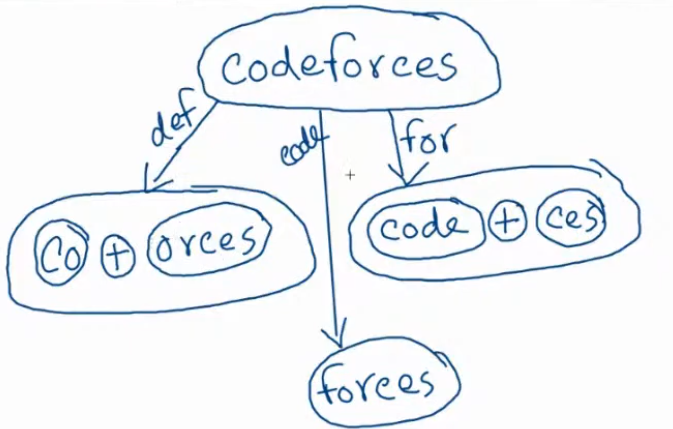
\includegraphics[width=0.5\linewidth]{images/grundy_tree.png}
\end{itemize}
}


\section{Misc.}
\subsection{\small [Trick] Median of Medians  \scriptsize}
\inputminted[breaklines, breakanywhere]{c++}{code/10-Misc./02-[Trick] Median of Medians.cpp}

{\footnotesize
\textbf{Problem:} Median of All Sub-Array Medians \\
\textbf{Idea:} Total Subarray, $k = \frac{n(n + 1)}{2}$. We need all subarray medians, sort them and get $\frac{k}{2}+1$. Now, Binary Search on Answer. ok() will return true if $cnt >= \frac{k}{2}+1$, where $cnt=$ count of subarrays whose median is $<=mid$. If true, $r=mid-1$
}

\subsection{\small Ternary Search  \scriptsize}
\inputminted[breaklines, breakanywhere]{c++}{code/10-Misc./04-Ternary Search.cpp}

\subsection{\small Pigeonhole Principle  \scriptsize}
\inputminted[breaklines, breakanywhere]{c++}{code/10-Misc./05-Pigeonhole Principle.cpp}

{\footnotesize
\begin{itemize}
\item At least 1 subarray of an array of length $N$ must be divisible by $N$.
\item Build all possible sequences of length 10 whose value is between 1 to 100. At least any two sequences will be same.
\item For $N>=100$, at least one 4-tuples XOR is 0.
\item For $N>20$ and $a_i<=10^6$, at least two subsets has same XOR. Because distinct XOR count can be $10^6$ and Total Subset $2^{20}>10^6$. Means there is a subset whose XOR is 0.
\end{itemize}
}


\subsection{\small Matrix Expo  \scriptsize}
\inputminted[breaklines, breakanywhere]{c++}{code/10-Misc./07-Matrix Expo.cpp}

\subsection{\small 2D Prefix Sum  \scriptsize}
\inputminted[breaklines, breakanywhere]{c++}{code/10-Misc./08-2D Prefix Sum.cpp}

\subsection{\small 2D Static Range Update  \scriptsize}
\inputminted[breaklines, breakanywhere]{c++}{code/10-Misc./09-2D Static Range Update.cpp}

\subsection{\small CHECK SET CLR  \scriptsize}
\inputminted[breaklines, breakanywhere]{c++}{code/10-Misc./10-CHECK SET CLR.cpp}

\subsection{\small Graph Directions  \scriptsize}
\inputminted[breaklines, breakanywhere]{c++}{code/10-Misc./11-Graph Directions.cpp}

\subsection{\small Custom Hash  \scriptsize}
\inputminted[breaklines, breakanywhere]{c++}{code/10-Misc./12-Custom Hash.cpp}

\subsection{\small Coordinate Compression  \scriptsize}
\inputminted[breaklines, breakanywhere]{c++}{code/10-Misc./13-Coordinate Compression.cpp}

\subsection{\small Submask Generator  \scriptsize}
\inputminted[breaklines, breakanywhere]{c++}{code/10-Misc./14-Submask Generator.cpp}

\subsection{\small Custom Comparators  \scriptsize}
\inputminted[breaklines, breakanywhere]{c++}{code/10-Misc./15-Custom Comparators.cpp}

\subsection{\small MOD Operations  \scriptsize}
\inputminted[breaklines, breakanywhere]{c++}{code/10-Misc./16-MOD Operations.cpp}

\subsection{\small Mex with Array Updates  \scriptsize}
\inputminted[breaklines, breakanywhere]{c++}{code/10-Misc./17-Mex with Array Updates.cpp}

\subsection{\small Check Eq AlphaQ  \scriptsize}
\inputminted[breaklines, breakanywhere]{c++}{code/10-Misc./18-Check Eq AlphaQ.cpp}

\section{Geometry}
\subsection{\small Convex Hull  \scriptsize}
\inputminted[breaklines, breakanywhere]{c++}{code/11-Geometry/01-Convex Hull.cpp}

\subsection{\small Area of 2 polygon intersection  \scriptsize}
\inputminted[breaklines, breakanywhere]{c++}{code/11-Geometry/02-Area of 2 polygon intersection.cpp}

\subsection{\small Point Segment Distance  \scriptsize}
\inputminted[breaklines, breakanywhere]{c++}{code/11-Geometry/03-Point Segment Distance.cpp}

\subsection{\small Three Point Circle  \scriptsize}
\inputminted[breaklines, breakanywhere]{c++}{code/11-Geometry/04-Three Point Circle.cpp}

\subsection{\small Circle Line Intersection  \scriptsize}
\inputminted[breaklines, breakanywhere]{c++}{code/11-Geometry/05-Circle Line Intersection.cpp}

{\footnotesize
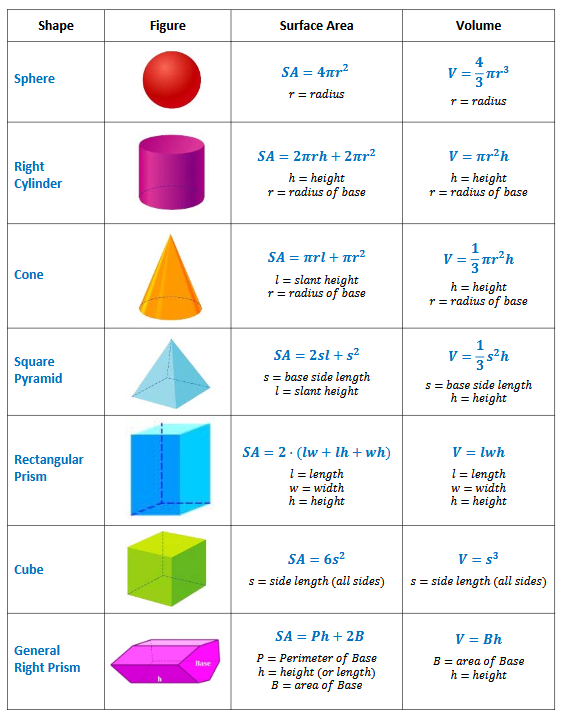
\includegraphics[width=0.7\linewidth]{images/shape-image-2.png}\\
% 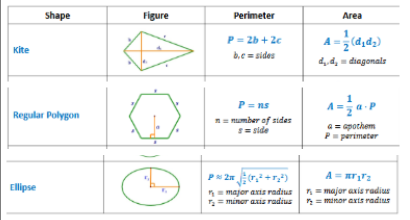
\includegraphics[width=1\linewidth]{images/shape-image-3.png}
\begin{center}
\footnotesize % Using the font size you specified
\begin{tabular}{|c|p{1.9cm}|c|c|}
\hline
\textbf{Shape} & \textbf{Figure} & \textbf{Perimeter} & \textbf{Area} \\
\hline
Kite & \begin{tabular}{@{}l@{}}  \\ $b, c$ = sides \\ $d_1, d_2$ = diagonals \end{tabular} & $P = 2b + 2c$ & $A = \frac{1}{2}(d_1 d_2)$ \\
\hline
Polygon & \begin{tabular}{@{}l@{}}  \\ $n = \text{number of sides}$ \\ $s = \text{side}$ \\ $a = \text{apothem}$ \\ $P = \text{perimeter}$ \end{tabular} & $P = ns$ & $A = \frac{1}{2} a \cdot P$ \\
\hline
Ellipse & \begin{tabular}{@{}l@{}}  \\ $r_1 = \text{mx rad}$ \\ $r_2 = \text{mn rad}$ \end{tabular} & $P \approx 2\pi \sqrt{\frac{1}{2}(r_1^2 + r_2^2)}$ & $A = \pi r_1 r_2$ \\
\hline
\end{tabular}
\end{center}
}

